\documentclass[a4paper]{article}

\usepackage[utf8]{inputenc}
\usepackage[portuguese]{babel}
\usepackage{a4wide}
\usepackage[pdftex]{hyperref}
\usepackage{graphicx}
\usepackage{wrapfig}
\usepackage{amsmath}
\usepackage{verbatim}
\usepackage{caption}
\usepackage{subcaption}
\usepackage{float}



\begin{document}

\begin{titlepage}
\begin{center}



\includegraphics[width=0.6\textwidth]{logo.jpg}\\[0.5cm]

{\large Universidade do Minho - Escola de Engenharia}\\[0.5cm]

{\large Relatório do trabalho prático de Sistemas Distribuídos}\\[0.5cm]

% Title
\rule{\linewidth}{0.5mm} \\[0.4cm]
{ \huge \bfseries Matchmaking num jogo online \\[0.4cm] }
\rule{\linewidth}{0.5mm} \\[1.5cm]

% Author and supervisor
\noindent
\begin{minipage}{0.4\textwidth}
  \begin{flushleft} \large
    \emph{Autores :}\\
    Daniel Maia \textsc{(A77531)}\\
    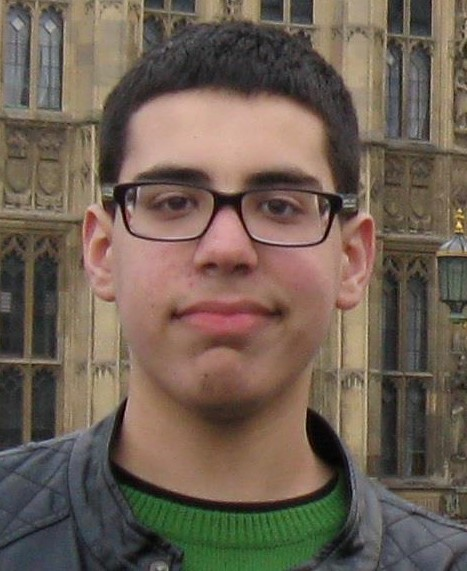
\includegraphics[width=1.5cm]{daniel.jpg}\break
    Diogo Silva\textsc{(A78034)}\\
    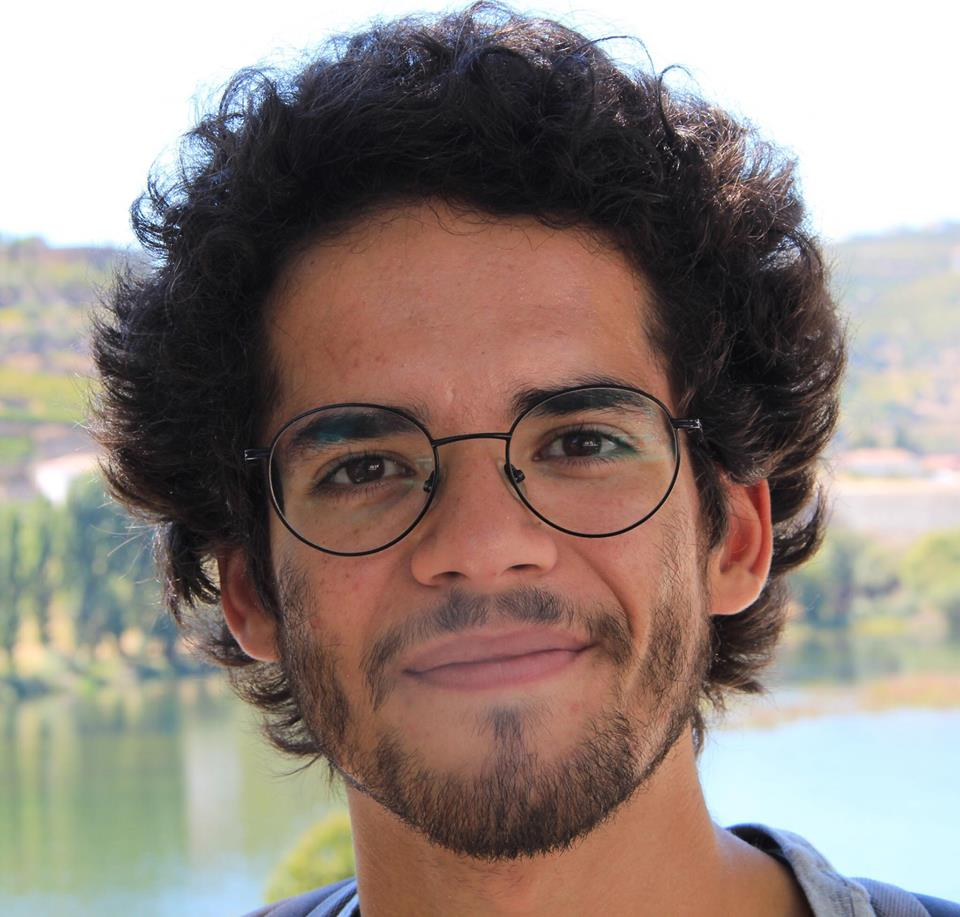
\includegraphics[width=1.5cm]{afonso.jpg}\break
    Marco Silva\textsc{(A79607)}\\
    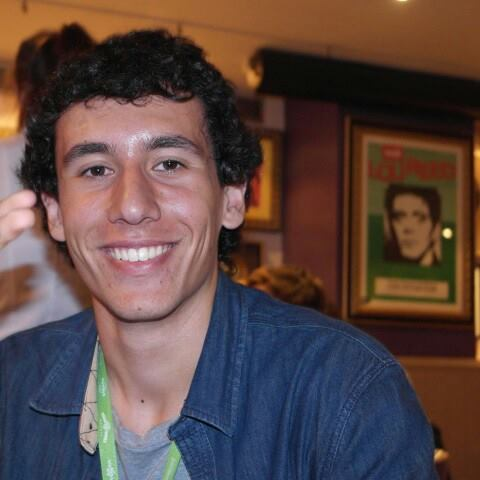
\includegraphics[width=1.5cm]{marco.jpg}\break
  \end{flushleft}
\end{minipage}%
\vfill

% Bottom of the page
{\large Versão 1.0 \\ \today}

\end{center}
\end{titlepage}




\begin{abstract}

\hspace{3mm} 

\end{abstract}

\pagebreak
\tableofcontents

\pagebreak
\section{Introdução}
\label{sec:1}

\hspace{3mm} 



%------------------------------------------------------------------------

\pagebreak
\section{Descrição do problema}
\label{sec:2}

\hspace{3mm}


\pagebreak
\clearpage
%--------------------------------------------------------------------------

\section{Conceção da Solução}
\label{sec:3}

\subsection{Registo e login}

\hspace{3mm} 



\subsection{Matchmaking}

\hspace{3mm} 


\subsection{Fazer equipas}

\hspace{3mm} 

\subsection{Escolha de heróis}

\hspace{3mm} A fase de escolha dos heróis permite aos jogadores escolherem os heróis com os quais pretendem jogar. No entanto, essa escolha deve ser transmitida para todos os jogadores da sua equipa para que estes tomem conhecimento da decisão. Os jogadores que pertencem à mesma partida mas à equipa contrária não devem ter acesso à conversação realizada pela equipa contrária.

Desta forma, a solução que permite implementar esta funcionalidade é constituída por um \texttt{ChatEscolhaHerois}, um \texttt{Timer}, um \texttt{TrataJogadorEscrita}, um \texttt{TrataJogadorLeitura} e um \texttt{ClientWorker}. Na realidade a classe \texttt{ChatEscolhaHerois} encontra-se armazenada pelo número da sala e número de partida numa estrutura definida pela classe \texttt{HashChats}. Esta classe classe organiza cada chat de acordo com o número da sala e partida, visto que estes dois valores identificam únicamente uma partida. Para tal utiliza a seguinte estrutura: \texttt{Map<Integer, Map<Integer, ChatEscolhaHerois>>}. Na prática todas as threads confirmam que já têm um chat pronto para o seu jogo. A primeira thread a perceber que ainda não existe, ficam incumbida de criar uma instância da classe \texttt{ChatEscolhaHerois} e coloca-la na \textit{hash}. As restantes threads apenas acedem ao chat criado.

%ChatEscolhaHerois
A classe \texttt{ChatEscolhaHerois} é responsável por armazenar toda a informação relacionada com o chat, assim como com a escolha dos heróis. Deste modo, são utilizadas dois \textit{HashMaps}, um para cada equipa visto que os heróis entre equipas podem repetir, com uma chave identificada pelo nome do herói escolhido e o valor com o username do jogador que o escolheu. Cada \textit{HashMap} tem um \textit{lock} pois é uma estrutura partilhada por várias \textit{threads}, que sofre múltiplas inserções e remoções concorrentemente. O método de exclusão mútua utilizado para proteger os \textit{HashMaps} anteriores foi conseguido com a ajuda dos \textit{ReentrantLocks}, um por cada \textit{Map}. Efetivamente, esta decisão adveio do facto do método \texttt{escolheHeroi} ser utilizado pelas duas equipas indiferenciadamente. Caso este método fosse colocado como \texttt{synchronized} as duas equipas tornavam-se dependentes uma da outra na escolha dos heróis. Com os \textit{locks} consegue-se isolar a escolha das duas equipas, ou seja, enquanto uma equipa escolhe um herói a outra pode estar a fazê-lo visto que escrevem em estruturas diferentes, apenas utilizam o mesmo método, sendo que dentro da mesma equipa a concorrência é controlada e apenas um jogador de cada vez consuma a sua escolha. 
%Esta parte ainda tenho que ver porque deviamos ter um chat para cada equipa!!!
Além disso, a classe conta com a variável \texttt{log} do tipo \texttt{ArrayList<String>}, que é responsável por armazenar a conversa...


%TrataJogadorEscrita/Leitura & Estrutura utilizada
As classes \texttt{TrataJogadorEscrita} e \texttt{TrataJogadorLeitura} são o resultado do método utilizado para implementar comunicação entre o jogador e o servidor de forma a obter um chat funcional. Efetivamente, o \texttt{TrataJogadorEscrita} é responsável por ler da variável \texttt{log} mencionada acima, ou seja, do chat e transmiti-la para o jogador que lhe corresponde. Na verdade, a thread que anima esta classe encontra-se adormecida enquanto não existe alteração no chat. Mal um nova entrada seja introduzida, a thread acorda e reencaminha as novas entradas. Dado que cada jogador tem o seu \texttt{TrataJogadorEscrita} então é feito o \textit{broadcast} da informação do chat para todos os jogadores. A classe \texttt{TrataJogadorLeitura} é responsável maioritariamente por ler o herói escolhido pelo jogador e enviá-lo para o \texttt{log}. Além disso, realiza algum processamento nos dados que recebe do jogador, nomeadamente se este escolheu um herói que se encontra indisponível no momento é de imediato dito ao cliente que tem de refazer a sua escolha.

A classe \texttt{Timer} tem uma instância para cada partida. O objetivo desta é não deixar que a escolha dos heróis ultrapasse os trinta segundos. Cada instância é guardada numa hash que tem como chaves a sala e a partida. À semelhança do que acontece com o chat, a primeira thread a perceber que ainda não foi criado um \texttt{Timer} para a sua partida procede à sua criação. No final dos trinta segundos é colocado uma mensagem no chat para que esta ao ser difundida vá terminando todas as threads envolvidas no chat.

Além disso, no lado do jogador além da classe \texttt{Cliente} é cridada um \texttt{ClientWorker}. Este fica apenas responsável por ler o que vem do servidor e imprime no ecrã do jogador.

Reunindo todos os recursos é possível perceber pela figura \ref{} a conjugação de todos os componentes que o chat envolve. 

Inicialmente, é criada a estrutura do chat. De seguida são criadas as threads \texttt{TrataJogadorEscrita}, \texttt{TrataJogadorLeitura} e do \texttt{Timer}. Do lado do cliente é criado o \texttt{ClientWorker}. Neste momento o jogador encontra-se na posição de escolher o herói com o qual pretende jogar e envia a sua escolha ao \texttt{TrataJogadorLeitura}. Após processar o pedido do jogador, se estiver tudo correto, este é enviado ao \texttt{ChatEscolhaHerois} para que este efetiva a escolha do jogador. De seguida, acorda todas as threads do \texttt{TrataJogadorEscrita} e estas enviam a escolha do jogador a todos os outros jogadores da mesma equipa. Quando essa informação chega ao \texttt{ClientWorker} este simplesmente imprime a escolha no ecrã do jogador.

No final dos trinta segundos, a thread responsável por animar o \texttt{Timer} envio o código \textbf{timeout} ao chat para que este saiba que o tempo de escolha dos heróis acabou. Consequentemente, a thread \texttt{TrataJogadorEscrita} acorda com a nova entrada e confirma que todos os jogadores escolheram um herói. Caso alguém não tenha escolhido, então a variável \texttt{jogar} é colocada a \texttt{false} e o código \textbf{timeout} é enviado para o \texttt{ClientWorker}. Caso contrário, a variável \texttt{start} é colocada a \texttt{true} e o código \textbf{start} é enviado ao \texttt{ClientWorker}. No final a thread do \texttt{TrataJogadorEscrita} termina. O \texttt{ClientWorker} recebe o código e consoante o seu valor coloca ou não a variável jogar do lado do jogador a \texttt{true}. De seguida, envia o código \textbf{morre} ao \texttt{TrataJogadorLeitura} para este terminar e ambos terminam a sua execução.

%Figura do esquema geral

\subsection{Cálculo dos resultados}

\hspace{3mm} O cálculo de resultados é realizado de forma aleatória dado que não se encontra implementado o jogo propriamente.

De facto, a classe que armazena todas as instâncias de \texttt{Jogo} é a \texttt{HashJogos}. Mais uma vez, à semelhança do que acontece com o chat utiliza-se um \textit{HashMap} com as chaves sendo a sala e a partida, para armazenar todos os jogos que são realizados. A primeira thread cria a instância de jogo. A última coloca o jogo a correr, ou seja, é a que dispulta o cálculo do resultado. Para o efeito é usado a expressão \texttt{this.resultado = (Math.random()<0.5)?1:2;}, que permite obter um resultado aleatório entre 1 e 2. Sendo que 1 significa que a equipa 1 ganhou e 2 significa que a equipa 2 ganhou. 

Por fim, o resultado é guardado na instância de Jogo para mais tarde ser consultado e consequentemente enviado para o jogador.

\pagebreak

%--------------------------------------------------------------------------

\section{Conclusões}
\label{sec:4}

\hspace{3mm} 



\end{document}
